\documentclass[25pt, a0paper, portrait]{tikzposter}
% \documentclass{tikzposter}
% \geometry{paperwidth=36in,paperheight=44in}
\makeatletter
\setlength{\TP@visibletextwidth}{\textwidth-2\TP@innermargin}
\setlength{\TP@visibletextheight}{\textheight-2\TP@innermargin}
\makeatother


\makeatletter
\newcommand\insertlogoi[2][]{\def\@insertlogoi{\includegraphics[#1]{#2}}}
\newcommand\insertlogoii[2][]{\def\@insertlogoii{\includegraphics[#1]{#2}}}
\newcommand{\tikzpar}{\setlength{\parindent}{5ex}}
\newlength\LogoSep
\setlength\LogoSep{-100pt}

\insertlogoi[width=7cm]{src/D-Pine.eps}
\insertlogoii[width=7cm]{src/Figures/logo_white.png}
% \usetheme{Simple}

\newcounter{tablecounter}
\newenvironment{tikztable}[1][]{
  \def \rememberparameter{#1}
  \vspace{10pt}
  \refstepcounter{tablecounter}
  \begin{center}
  }{
    \ifx\rememberparameter\@empty
    \else
    \\[10pt]
    {\small Tab.~\thetablecounter: \rememberparameter}
    \fi
  \end{center}
}


\renewcommand\maketitle[1][]{  % #1 keys
    \normalsize
    \setkeys{title}{#1}
    % Title dummy to get title height
    \node[transparent,inner sep=\TP@titleinnersep, line width=\TP@titlelinewidth, anchor=north, minimum width=\TP@visibletextwidth-2\TP@titleinnersep]
        (TP@title) at ($(0, 0.5\textheight-\TP@titletotopverticalspace)$) {\parbox{\TP@titlewidth-2\TP@titleinnersep}{\TP@maketitle}};
    \draw let \p1 = ($(TP@title.north)-(TP@title.south)$) in node {
        \setlength{\TP@titleheight}{\y1}
        \setlength{\titleheight}{\y1}
        \global\TP@titleheight=\TP@titleheight
        \global\titleheight=\titleheight
    };

    % Compute title position
    \setlength{\titleposleft}{-0.5\titlewidth}
    \setlength{\titleposright}{\titleposleft+\titlewidth}
    \setlength{\titlepostop}{0.5\textheight-\TP@titletotopverticalspace}
    \setlength{\titleposbottom}{\titlepostop-\titleheight}

    % Title style (background)
    \TP@titlestyle

    % Title node
    \node[inner sep=\TP@titleinnersep, line width=\TP@titlelinewidth, anchor=north, minimum width=\TP@visibletextwidth-2\TP@titleinnersep]
        at (0,0.5\textheight-\TP@titletotopverticalspace)
        (title)
        {\parbox{\TP@titlewidth-2\TP@titleinnersep}{\TP@maketitle}};

    \node[inner sep=0pt,anchor=west] 
      at ([xshift=-\LogoSep]title.west)
      {\@insertlogoi};

    \node[inner sep=0pt,anchor=east] 
      at ([xshift=\LogoSep]title.east)
      {\@insertlogoii};

    % Settings for blocks
    \normalsize
    \setlength{\TP@blocktop}{\titleposbottom-\TP@titletoblockverticalspace}
}
\makeatother

\definecolorstyle{sampleColorStyle} {
	\definecolor{colorOne}{named}{white}
	\definecolor{colorTwo}{named}{red}
	\definecolor{colorThree}{named}{red}
	\definecolor{Dgreen}{HTML}{00693e}
}{
	% Background Colors
	\colorlet{backgroundcolor}{colorOne}
	\colorlet{framecolor}{white}
	% Title Colors
	\colorlet{titlefgcolor}{white}
	\colorlet{titlebgcolor}{Dgreen}
	% Block Colors
	\colorlet{blocktitlebgcolor}{white}
	\colorlet{blocktitlefgcolor}{Dgreen}
	\colorlet{blockbodybgcolor}{white}
	\colorlet{blockbodyfgcolor}{black}
	% Innerblock Colors
	\colorlet{innerblocktitlebgcolor}{white}
	\colorlet{innerblocktitlefgcolor}{black}
	\colorlet{innerblockbodybgcolor}{colorThree!30!white}
	\colorlet{innerblockbodyfgcolor}{black}
	% Note colors
	\colorlet{notefgcolor}{black}
	\colorlet{notebgcolor}{colorTwo!50!white}
	\colorlet{noteframecolor}{colorTwo}
}

\definelayouttheme{sample}{
	\usecolorstyle[colorPalette=sampleColorPalette]{sampleColorStyle}
	\usebackgroundstyle{sample}
	\usetitlestyle{Test}
	\useblockstyle{Simple}
	\useinnerblockstyle{Simple}
	\usenotestyle{Corner}
}

\usetheme{sample}

% \begin{document}
%\geometry{paperwidth=44in,paperheight=36in}
\usetitlestyle{Filled}
\title{
\begin{minipage}{\textwidth}
   \centering
   Chemically Self Consistent Isochrones
   \\
   \bigskip
   \mbox{of the Globular Cluster NGC 2808}
 \end{minipage}
 }
% \title{Updated High-Temperature Opacities for The Dartmouth Stellar Evolution Program and their Effect on the Jao Gap Location}
\author{Emily M. Boudreaux$^{1}$, Renata Edeas Hoh$^{1}$, Brian C. Chaboyer$^{1}$, \& Gregory Feiden$^{2}$}
\institute{{$^{1}$Department of Physics and Astronomy, Dartmouth College, Hanover, NH 03755, USA}\\{$^{2}$Department of Physics and Astronomy, University of North Georgia, Dahlonega, GA 30533, USA}}
\usepackage[utf8]{inputenc}
\usepackage{wrapfig}
\usepackage{amsmath}
\usepackage{setspace}
\usepackage{fontspec}
\usepackage[T1]{fontenc}
\usepackage{adjustbox}
\usepackage{tikz}
\usepackage{xcolor}

\tikzposterlatexaffectionproofoff

\begin{document}
	\maketitle
	\begin{columns}
	  \column{0.33}

		\block{Abstract}{\fontsize{38}{45}\selectfont
      \tikzpar The inferred helium mass fraction of multiple populations in
      globular clusters can vary signifigantly from older to younger populations.
      As the origin of these MPs remains an open question, and one which is
      sensitive to the population - population compositional differences, the
      extent of the composition variations is a key parameter when constraining
      formation channels. Many metal abundances may be directly measured
      spectroscopically; however, helium abundances are not directly observable
      in GCs. Instead, helium abundances are inferred from stellar models. It is
      therefore important to build stellar models which are chemically
      self-consistent between the structure, atmosphere, and opacities. In this
      work we present the first chemically self-consistent stellar models of the
      Milky Way Globular Cluster NGC 2808. We find that the helium abundance of
      the second generation of stars is higher than the first generation by SOME
      AMOUNT
      \vspace{-25mm}
    }

		\block{Updating Atmosphers}{\fontsize{38}{45}\selectfont
	    \vspace{-5mm}
			% \begin{tikzfigure}[Solar Calibrated Stellar Models using both OPAL
			% 	(black) and OPLIB (violet) high--temperature opacity tables.]
			% 	\includegraphics[width=0.28\textwidth]{src/Figures/NBFigs/HRDiagramOPALvsOPLIB_SCCM.pdf}
			% \end{tikzfigure}

			\tikzpar For much of a stars radius ($\log(R)\approx-1.5$), OPAL
			and OPLIB opacities vary by up to approximately 2\%. We calibrate a
			solar model (above) to confirm that variations of this order do not
			dramatically alter a solar model's evolutionary path.


			\tikzpar These small variations may be more impactful for stars at or near
			the convective transition mass. The interior structure, which is
			believed to result in the Jao Gap, of such stars is very sensitive
			to temperature; therefore, small changes in opacity may be more
			impactful than in higher mass models.
	    }
		\block{Updating Opacities}{\fontsize{38}{45}\selectfont
	    \vspace{-5mm}
			% \begin{tikzfigure}[Solar Calibrated Stellar Models using both OPAL
			% 	(black) and OPLIB (violet) high--temperature opacity tables.]
			% 	\includegraphics[width=0.28\textwidth]{src/Figures/NBFigs/HRDiagramOPALvsOPLIB_SCCM.pdf}
			% \end{tikzfigure}

			\tikzpar For much of a stars radius ($\log(R)\approx-1.5$), OPAL
			and OPLIB opacities vary by up to approximately 2\%. We calibrate a
			solar model (above) to confirm that variations of this order do not
			dramatically alter a solar model's evolutionary path.


			\tikzpar These small variations may be more impactful for stars at or near
			the convective transition mass. The interior structure, which is
			believed to result in the Jao Gap, of such stars is very sensitive
			to temperature; therefore, small changes in opacity may be more
			impactful than in higher mass models.
	    }

		\block{References}{
			\vspace{-1cm}
			\begin{minipage}[t]{0.75\linewidth}
				{\fontsize{24}{22}\selectfont
				\begin{enumerate}
					\item Dotter, A., Chaboyer, B., Jevremovi ́c, D., et al. 2008, The Astrophysical Journal Supplement Series, 178, 89 
					\item van Saders, J. L., \& Pinsonneault, M. H. 2012, The Astrophysical Journal, 751, 98
					\item Jao, W.-C., Henry, T. J., Gies, D. R., \& Hambly, N. C. 2018, ApJL, 861, L11,
				\end{enumerate}
				}
			\end{minipage}%
			\begin{adjustbox}{valign=t}
			\begin{minipage}[t]{0.25\linewidth}
				\hspace{5mm}
				% \includegraphics[scale=0.65]{src/QR.pdf}
			\end{minipage}
			\end{adjustbox}
			{\fontsize{24}{22}\selectfont
			\begin{enumerate}
				 \setcounter{enumi}{3}
				 \item Colgan, J., Kilcrease, D. P., Magee, N. H., et al. 2016, in APS Meeting Abstracts, Vol. 2016, APS Division of Atomic, Molecular and Optical Physics Meeting Abstracts, D1.008
			\end{enumerate}
			}
		}
	

	  \column{0.66}
    \block{Fiducial Measurment}{\fontsize{38}{45}\selectfont
      \tikzpar In order to measure the subtle number density variations seperating
      populations along the Main Sequence we make use of a novel, convex-hull
      based, adaptive binning approach. This algorithm keeps the number of stars
      per bin uniform. An example of the density estiamte produced by this
      algorithm is showin in Figure 1. Note how the sequences stand out clearly
      in the density plot.

      \begin{tikzfigure}[NGC 2808 CMD from the HUGS survey after data quality cuts have been applied (top). Number density of stars in the CMD of NGC 2808 (bottom). Darker regions are more dense.]
        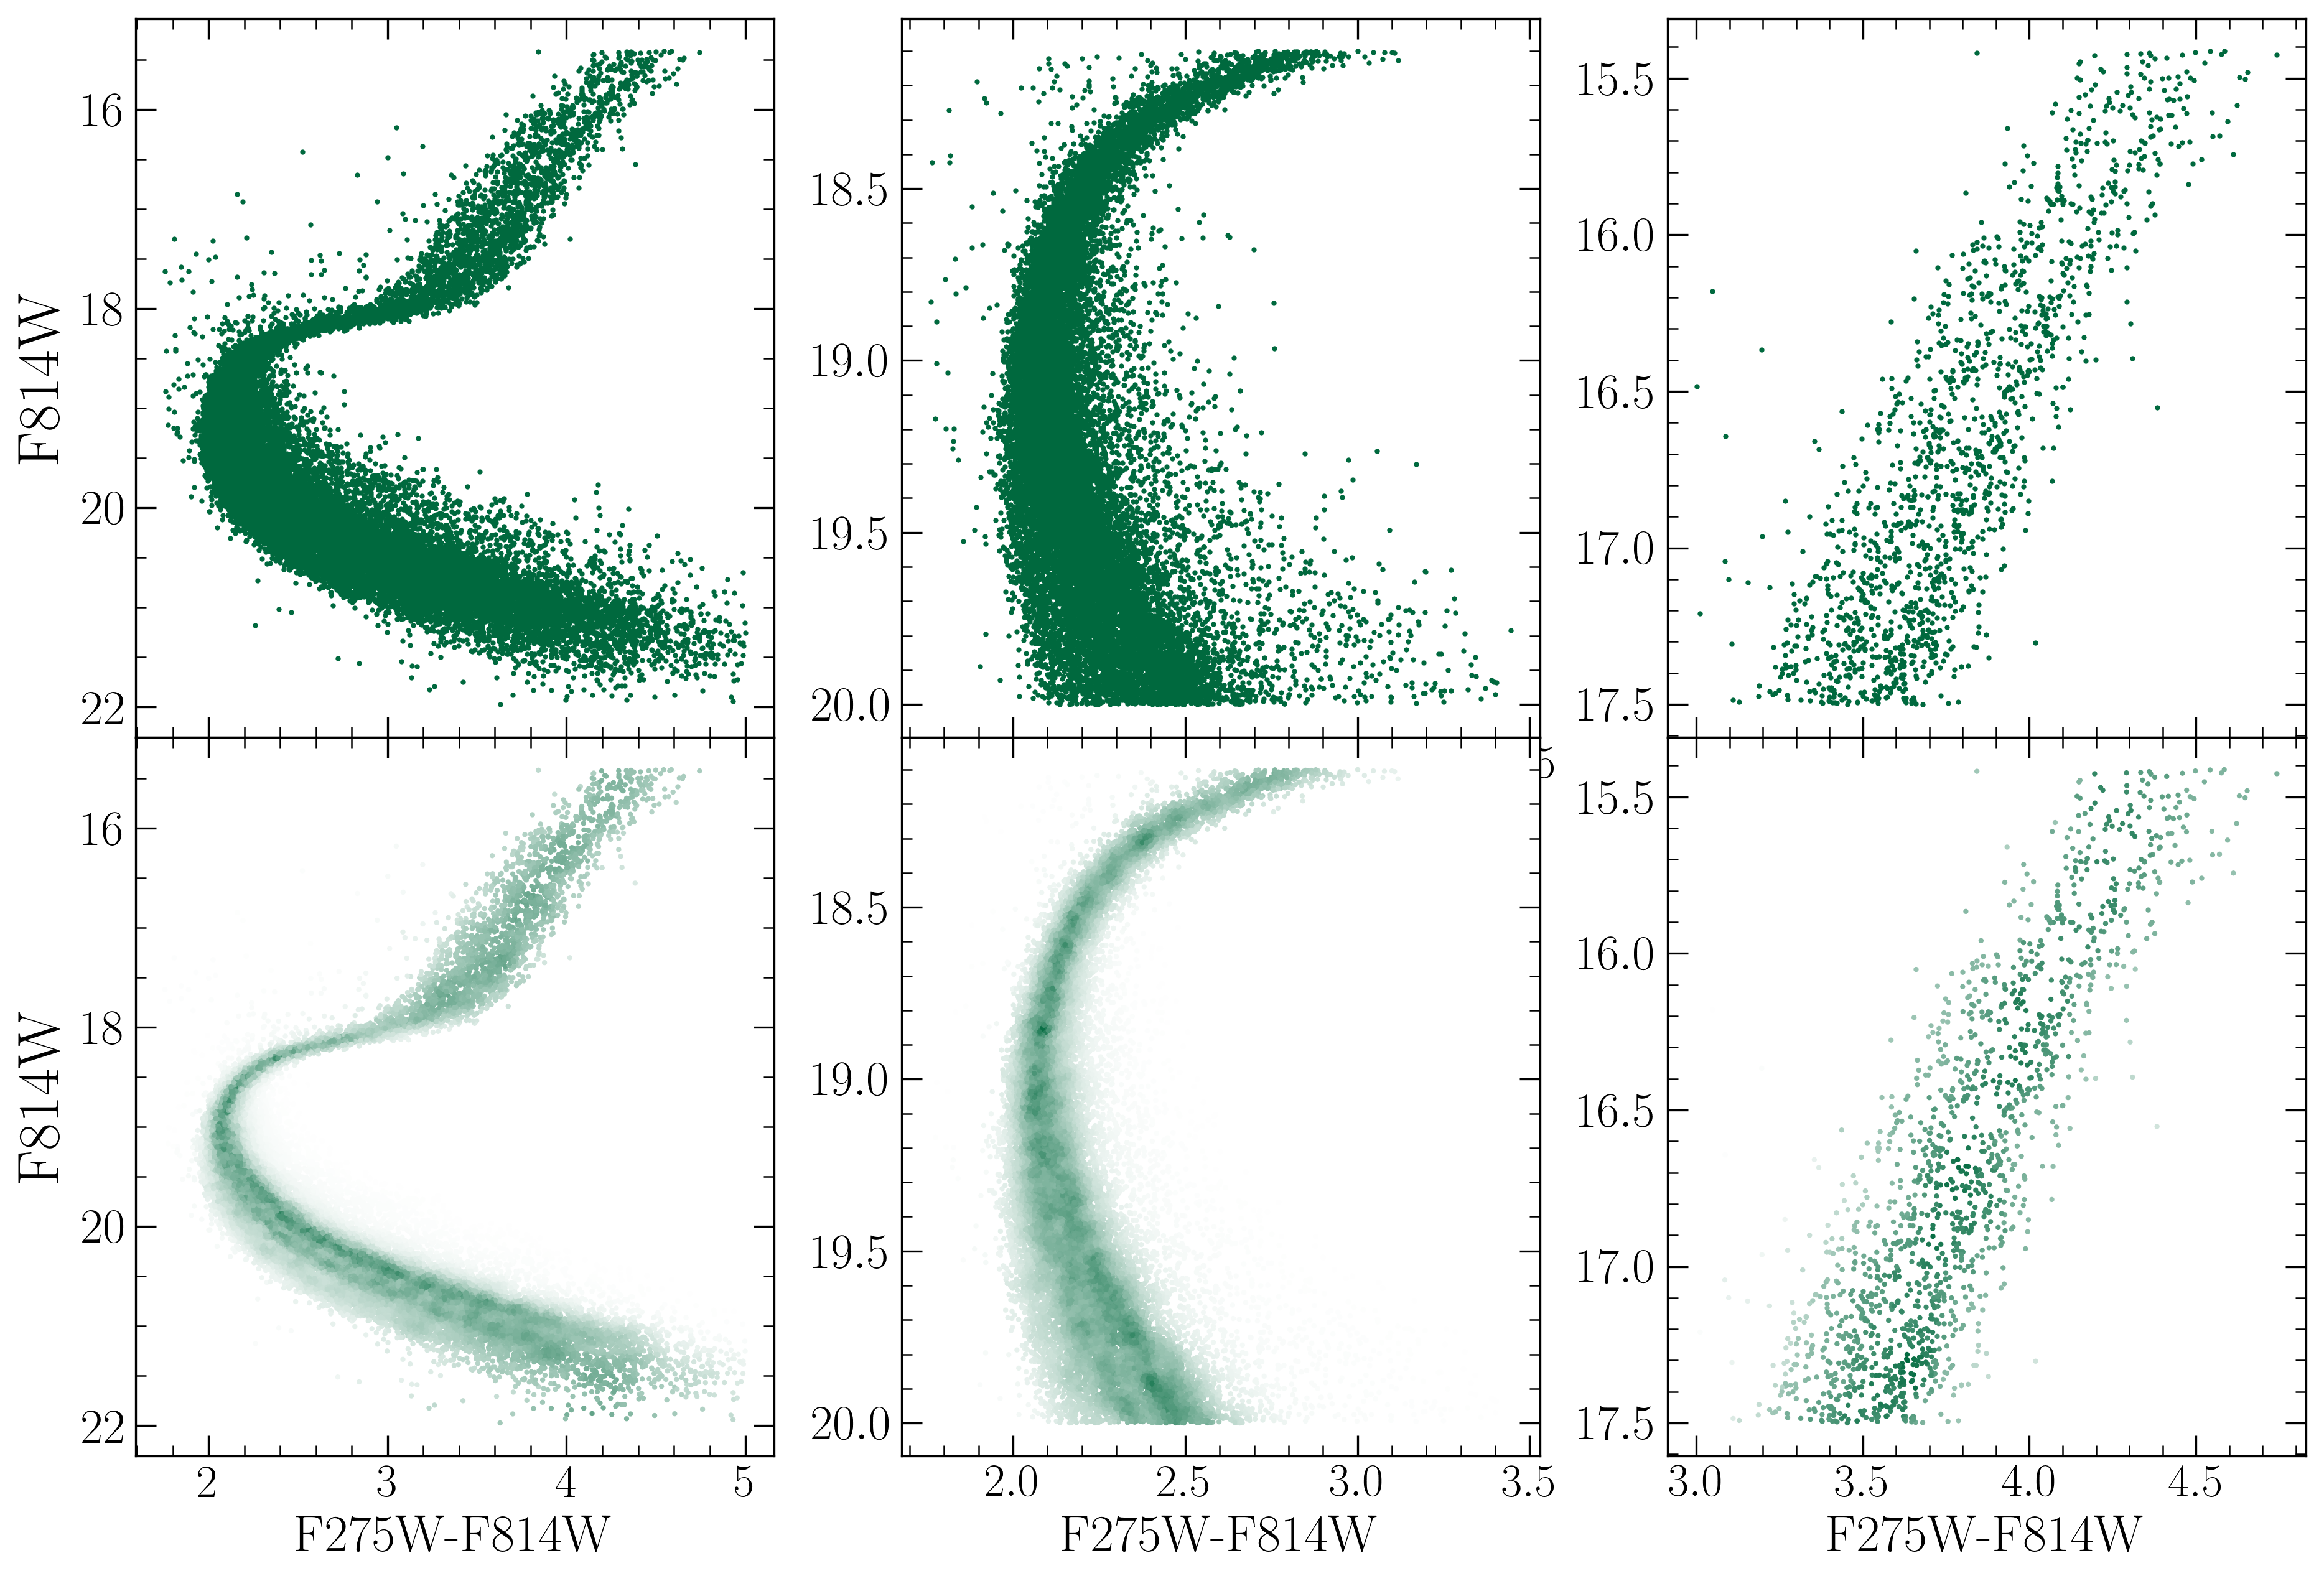
\includegraphics[width=0.6\textwidth]{src/Figures/NBFigs/DensityMap.png}
      \end{tikzfigure}

			\begin{minipage}[t]{0.33\linewidth}
      \tikzpar In order to trace the sequences we use Baysian Gaussian Mixture Modeling
      and the Diecrelt Process to fit the color-density profile over a series of
      magnitude bins. This eliminats the need for a prior on exact the number of
      populations, instead only requiring the max number of populations to be
      defined. Traced fiducial lines for NGC 2808 two most extreme populations
      (A\&E in Milone et al. 2015) are showin in Figure 2.
			\end{minipage}%
			\begin{adjustbox}{valign=t}
        \begin{minipage}[t]{0.66\linewidth}
          \begin{tikzfigure}[NGC 2808 populations A \& E median ridge lines measured using fidanka.]
            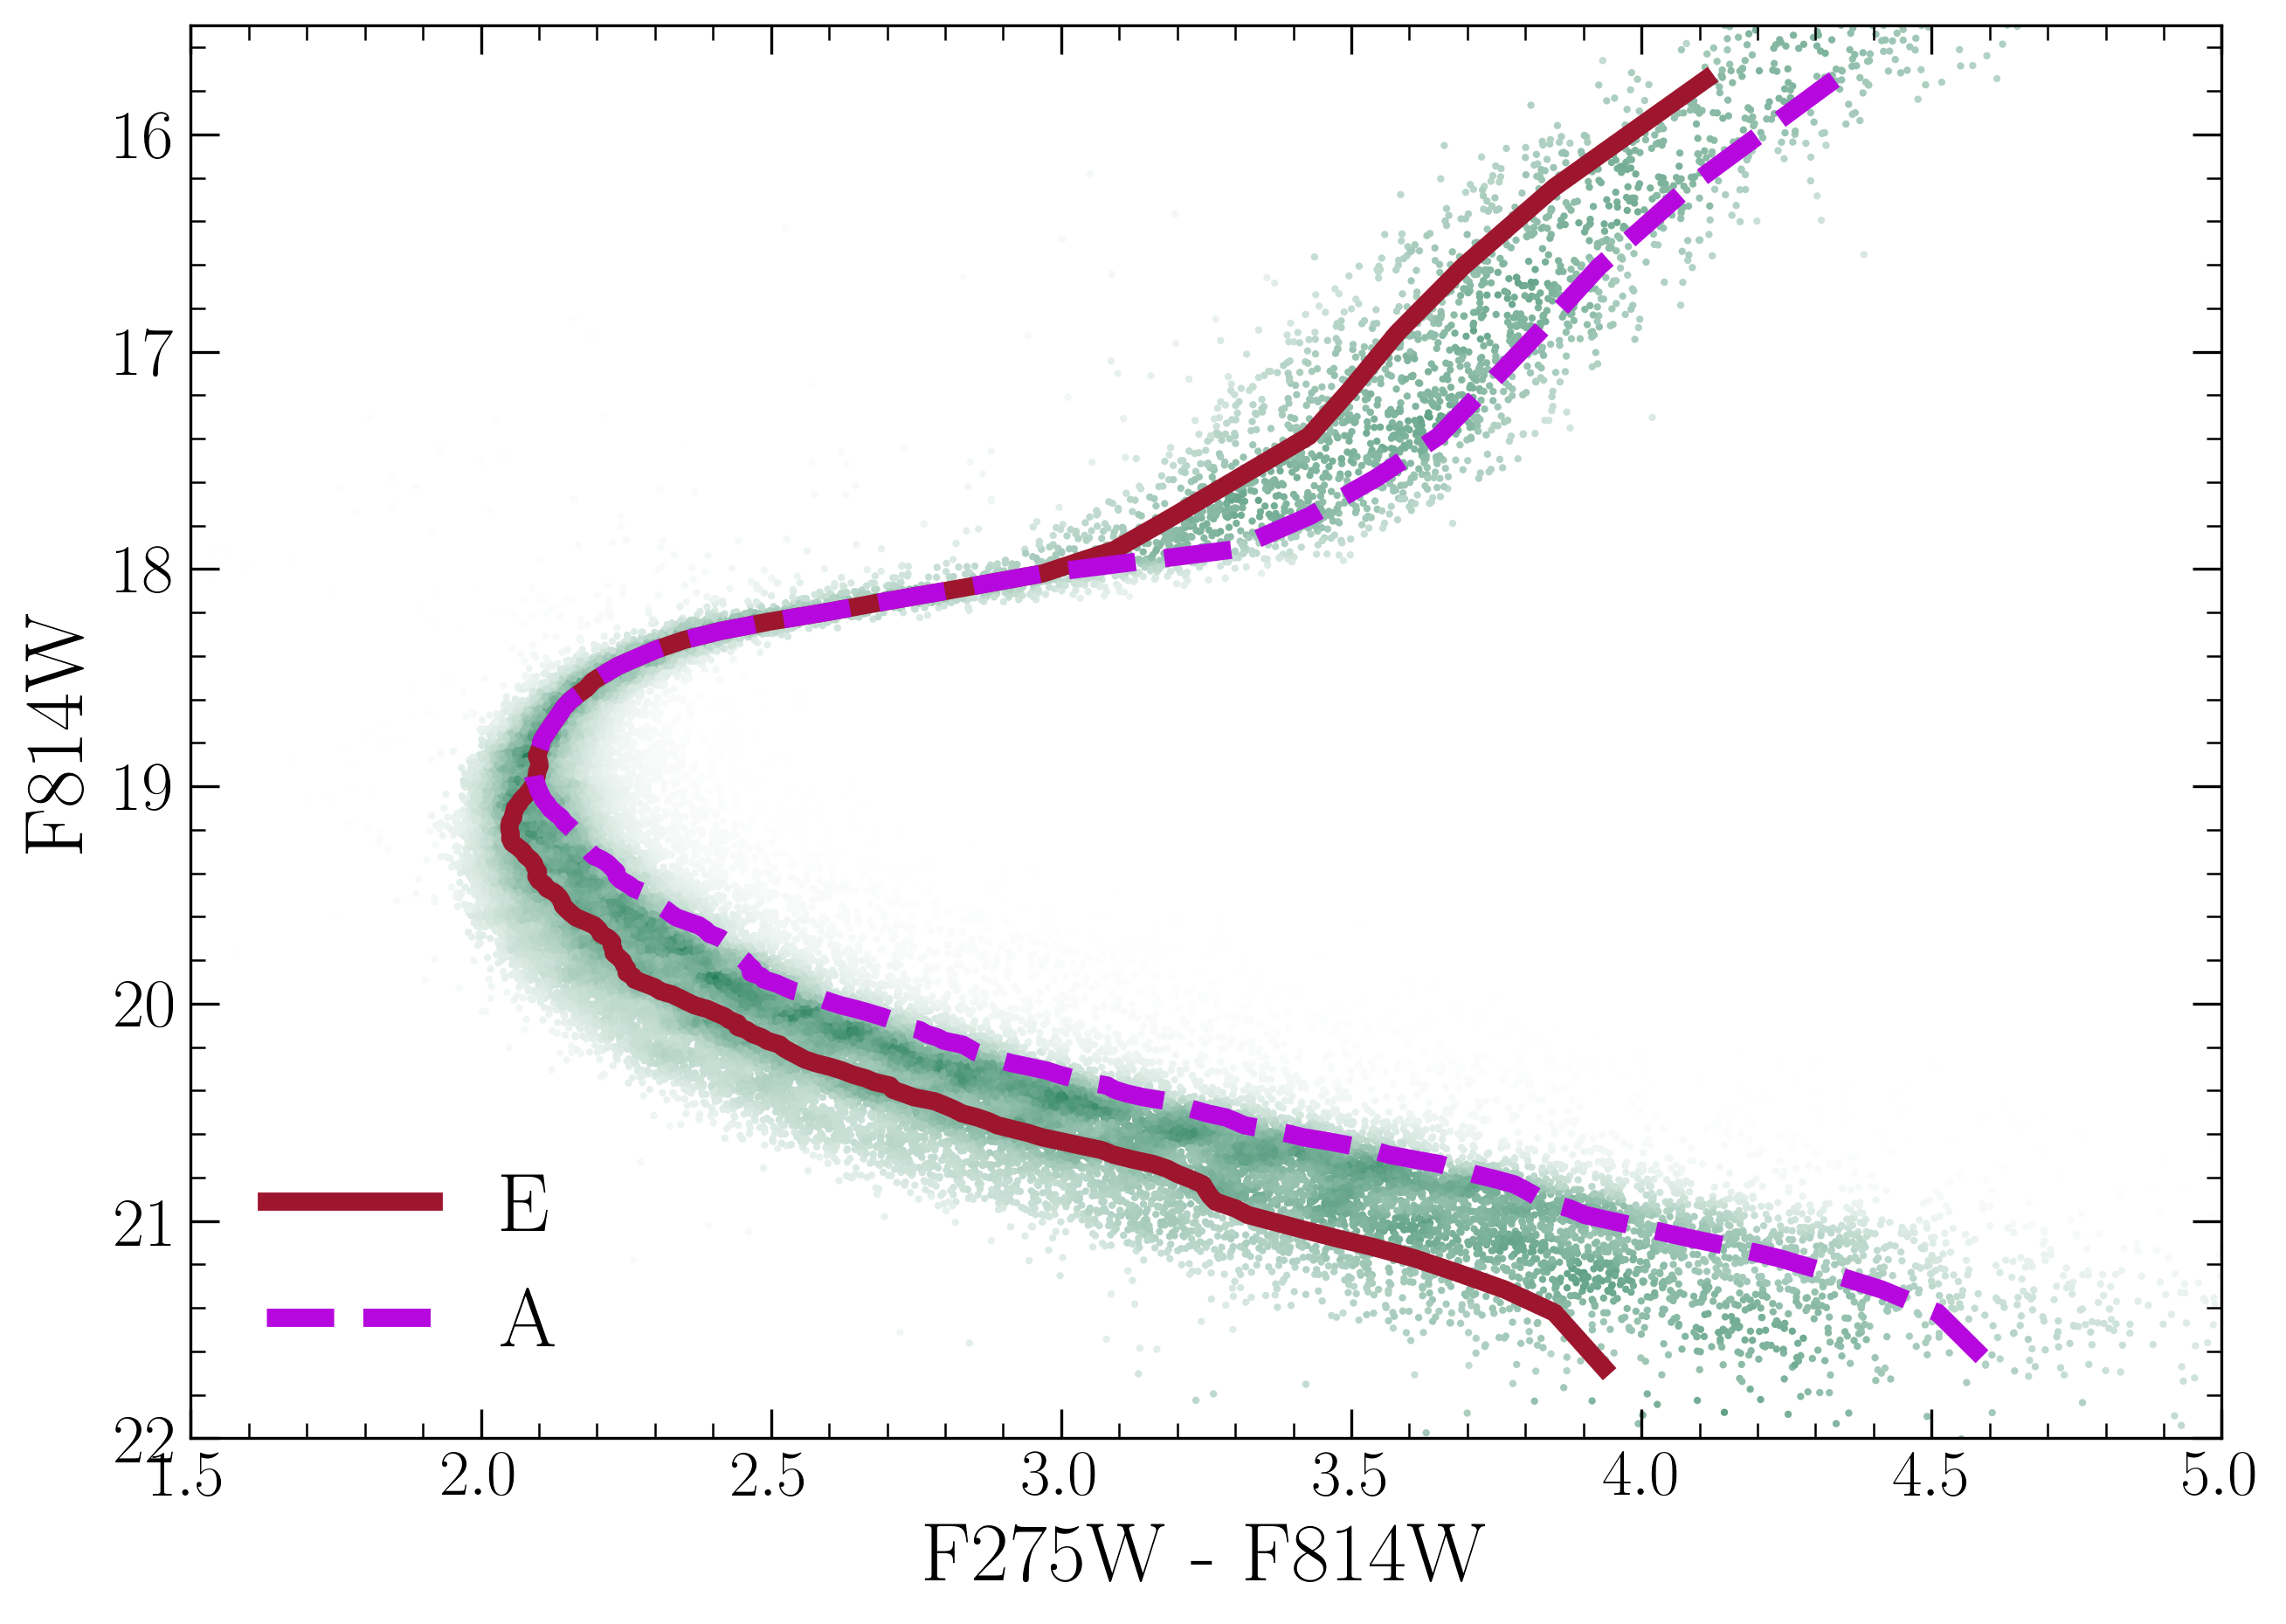
\includegraphics[scale=1]{src/Figures/NBFigs/NGC2808Fid.png}
          \end{tikzfigure}
        \end{minipage}
			\end{adjustbox}

    }
		% \block{Modeling the Gap}{\fontsize{38}{45}\selectfont
		% 	\tikzpar A theoretical explanation for the Jao Gap comes from
		% 	van Saders \& Pinsonneault 2012, who propose that in a star directly above the
		% 	transition mass, due to asymmetric production and destruction of
		% 	He$^{3}$ during the proton-proton I chain (ppI), periodic
		% 	luminosity variations can be induced. This is known
		% 	as convective-kissing instability.
		% 	

		% 	\vspace{-2cm}
	 %    }

  %     {\begin{center}
		% 		\bf{\color{Dgreen}\large Acknowledgments}
  %     \end{center}}

		% 	{
		% 	\fontsize{23}{20}\selectfont
		% 	We acknowledge the support of an NASA grant (No.
		% 	80NSSC18K0634). Additionally, we would like to thank James
		% 	Colgan for his assistance with the OPLIB opacity tables. We
		% 	would also like to thank Aaron Dotter and Elisabeth Newton.
		% 	}


	\end{columns}
\end{document}
